% =====================================================================
%  JuliaCon Global 2026 — Poster (portrait A0)
%  Using The HeartRateLab.jl for Normative Evaluation of Heart Rate
%  Variability from Open Datasets  ·  Alberto Barradas (abcsds)
%
%  Build:  pdflatex juliacon2026_poster.tex   (run twice for QR/refs)
%  Design system extracted from the JuliaCon 2026 brand
%  (github.com/JuliaCon/www.juliacon.org, franklin/_assets/2026).
% =====================================================================
\documentclass[fontsize=20pt]{scrartcl}

\usepackage[T1]{fontenc}
\usepackage[utf8]{inputenc}
\usepackage[sfdefault]{FiraSans}
\usepackage[paperwidth=841mm,paperheight=1189mm,top=15mm,bottom=12mm,left=18mm,right=18mm]{geometry}
\usepackage{tikz}
\usetikzlibrary{calc,positioning,shapes.geometric,backgrounds,fadings,arrows.meta}
\usepackage[most]{tcolorbox}
\usepackage{qrcode}
\usepackage{graphicx}
\usepackage{amsmath}
\usepackage{ragged2e}
\usepackage{fontawesome5}
\pagestyle{empty}
\setlength{\parindent}{0pt}

% ---------- JuliaCon / Julia brand palette ----------
\definecolor{jcindigo}{HTML}{38376C}   % primary bg
\definecolor{jcindigodk}{HTML}{201C46} % bg gradient bottom
\definecolor{jcpurple}{HTML}{4B518C}   % section rails
\definecolor{jclav}{HTML}{F3E8F2}      % light / footer band
\definecolor{jclavdk}{HTML}{D7D0DE}
\definecolor{jcgreen}{HTML}{389826}    % Julia green (typical / badge)
\definecolor{jured}{HTML}{CB3C33}      % Julia red (alert)
\definecolor{jupurple}{HTML}{9558B2}   % Julia purple
\definecolor{jublue}{HTML}{4063D8}     % Julia blue
\definecolor{zgold}{HTML}{E0A93B}      % slightly-atypical
\definecolor{cardnavy}{HTML}{2E2C57}
\definecolor{inkdark}{HTML}{23213F}

% ---------- tcolorbox styles ----------
\tcbset{
  card/.style={
    enhanced, colback=white, colframe=jcpurple,
    boxrule=0pt, arc=6mm, top=3.2mm, bottom=3.2mm, left=8mm, right=8mm,
    fontupper=\color{inkdark},
    borderline west={5mm}{0mm}{jcgreen},
    drop fuzzy shadow=black!35,
  },
  darkcard/.style={
    enhanced, colback=cardnavy, colframe=jcpurple,
    boxrule=0pt, arc=6mm, top=3.2mm, bottom=3.2mm, left=8mm, right=8mm,
    fontupper=\color{white},
    borderline west={5mm}{0mm}{jcgreen},
    drop fuzzy shadow=black!45,
  },
}
% card title macro
\newcommand{\ctitle}[2][jcgreen]{{\color{#1}\bfseries\LARGE #2}\par\vspace{4mm}}

% ---------- z-score forest plot ----------
% \zrow{ypos}{z}{dotcolor}{feature name}
\newcommand{\zrow}[4]{%
  \draw[gray!60,line width=2.4pt] (0,#2) -- (#3,#2);
  \fill[#4] (#3,#2) circle (8pt);
  \draw[white,line width=1pt] (#3,#2) circle (8pt);
  \node[anchor=east,text=white,font=\bfseries] at (-3.05,#2) {#1};
  \node[anchor=west,text=white,font=\bfseries] at (3.65,#2)
        {\pgfmathprintnumber[print sign,fixed,fixed zerofill,precision=2]{#3}$\sigma$};
}
% \zforest{max-y}{rows}  — draws bands + axis then the rows
\newcommand{\zforest}[2]{%
\begin{tikzpicture}[x=2.55cm,y=1.14cm]
  \def\ymax{#1}
  % dispersion bands
  \fill[jublue!22]  (-1,-0.55) rectangle (1,\ymax+0.55);
  \fill[zgold!26]   (-2,-0.55) rectangle (-1,\ymax+0.55);
  \fill[zgold!26]   (1,-0.55)  rectangle (2,\ymax+0.55);
  \fill[jured!16]   (-3,-0.55) rectangle (-2,\ymax+0.55);
  \fill[jured!16]   (2,-0.55)  rectangle (3.5,\ymax+0.55);
  % zero line + ticks
  \draw[white!85,dashed,line width=1.2pt] (0,-0.55) -- (0,\ymax+0.55);
  \foreach \t in {-2,-1,0,1,2,3}{
     \draw[white!45,line width=0.8pt] (\t,-0.55) -- (\t,-0.75);
     \node[below,text=white!80,font=\small] at (\t,-0.75) {\t};}
  \node[below,text=white!70,font=\small\itshape] at (0.5,-1.35)
        {z-equivalent (\,$\sigma$ from healthy-population median\,)};
  #2
\end{tikzpicture}}

% Julia dots (for juliacon wordmark)
\newcommand{\juliadots}[1]{%
\begin{tikzpicture}[scale=#1]
  \fill[jcgreen]  (0,0.52) circle (0.3);
  \fill[jublue]   (-0.45,0) circle (0.3);
  \fill[jured]    (0,0) circle (0.3);
  \fill[jupurple] (0.45,0) circle (0.3);
\end{tikzpicture}}

\begin{document}
% ================= FULL-PAGE BACKGROUND =================
\begin{tikzpicture}[remember picture,overlay]
  \shade[top color=jcindigo,bottom color=jcindigodk]
        (current page.north west) rectangle (current page.south east);
  % subtle bubble texture
  \pgfmathsetseed{2026}
  \foreach \i in {1,...,150}{
    \pgfmathsetmacro{\rx}{rnd*841-420}
    \pgfmathsetmacro{\ry}{rnd*1189-620}
    \pgfmathsetmacro{\rr}{6+rnd*26}
    \pgfmathsetmacro{\ro}{2+rnd*6}
    \fill[white,opacity=\ro/100] ($(current page.center)+(\rx mm,\ry mm)$) circle (\rr mm);
    \draw[white,opacity=\ro/120,line width=0.4mm]
         ($(current page.center)+(\rx mm,\ry mm)$) circle (\rr mm);
  }
  % lavender footer band
  \fill[jclav] (current page.south west) rectangle
       ([yshift=95mm]current page.south east);
  \fill[jclavdk] ([yshift=95mm]current page.south west) rectangle
       ([yshift=98mm]current page.south east);
\end{tikzpicture}

% ================= HEADER =================
\vspace{-6mm}
\begin{minipage}[t]{0.775\linewidth}
  \raggedright
  {\setlength{\fboxsep}{6pt}\colorbox{jcgreen}{\color{white}\bfseries\Large\ POSTER\ }}\\[3mm]
  {\color{white}\bfseries\fontsize{52}{57}\selectfont
   Using The HeartRateLab.jl for\\ Normative Evaluation of Heart\\ Rate Variability
   from Open Datasets}\\[3mm]
  {\color{jclav}\Large\bfseries Luis Alberto Barradas Chacón}\quad
  {\color{white!75}\large Technische Universität Graz, Medizinische Universität Graz}
\end{minipage}\hfill
\begin{minipage}[t]{0.20\linewidth}
  \raggedleft
  \vspace{4mm}
  \begin{tcolorbox}[enhanced,colback=white,colframe=white,boxrule=0pt,arc=4mm,
       width=52mm,height=52mm,halign=center,valign=center,left=3mm,right=3mm,top=3mm,bottom=3mm]
     \qrcode[height=44mm]{https://github.com/abcsds/HeartRateLab.jl}
  \end{tcolorbox}\par\vspace{4mm}
  {\color{white!85}\small\bfseries github.com/abcsds/HeartRateLab.jl}
\end{minipage}

\vspace{4mm}

% ================= ABSTRACT + DESCRIPTION =================
\noindent
\begin{minipage}[t]{0.655\linewidth}
  \begin{tcolorbox}[card]
     \ctitle{Abstract}
     {
     A common method in the evaluation of human biosignals is contrasting a recording
     against reference datasets of similar experiments. Thanks to the open scientific
     resources for heart rate analysis, and the resilient network of scientific
     programming functionality that the Julia community enables, this \textbf{normative
     evaluation} of Heart Rate Variability (HRV) can be done \textbf{completely in Julia}.
     We score each \textbf{360-beat} window of a longitudinal self-tracked participant
     (\textbf{P1}) who practises \textbf{resonant breathing} against per-feature priors
     fitted to \textbf{61{,}715 windows from 66 healthy subjects} (PhysioNet
     \emph{nsrdb}+\emph{nsr2db}). Against this general population P1's low-frequency band
     is strongly elevated: \textbf{LF/HF} (z\,$=\!+2.6$), \textbf{LF power}
     (z\,$=\!+2.5$); while short-term vagal tone (\textbf{RMSSD} z\,$=\!+0.0$,
     \textbf{Mean IBI} z\,$=\!+0.1$) stays at the healthy median. Re-scored against
     \emph{meditators} (\emph{Heart Rate Oscillations during Meditation}, 11 practitioners,
     themselves only mildly shifted from healthy: pNN50 z\,$=\!+0.4$, SDNN
     z\,$=\!+0.8$), P1's elevation roughly halves (\textbf{LF/HF} z\,$=\!+1.7$): paced
     resonant breathing places P1 \emph{atypical} for the general population but
     \emph{meditator-like}. A recording is ``normal'' only relative to a chosen reference.
     In this way we demonstrate how correctly implemented open science can answer contextual
     questions such as: \emph{``Is this new experimental data normal?''}}
  \end{tcolorbox}
\end{minipage}\hfill
\begin{minipage}[t]{0.325\linewidth}
  \begin{tcolorbox}[card, borderline west={5mm}{0mm}{jublue}]
     \ctitle[jublue]{Why context matters}
     {
     We contrast a time series of \textbf{Inter-Beat Intervals (IBIs)} against the
     feature distributions of existing open datasets, emphasising the
     \textbf{contextual nature} of scientific inquiry. This capability is a novel
     addition implemented specifically for HeartRateLab.jl.\par\vspace{4mm}
     An example contrasting meditation recordings demonstrates current capabilities
     and illustrates functionality that aids \textbf{hypothesis testing},
     \textbf{feature engineering}, and a deeper understanding of recordings,
     including use as a \textbf{personal daily HRV monitor} that norms your own
     signals against a healthy population.}
  \end{tcolorbox}
\end{minipage}

\vspace{4mm}

% ================= COMPUTATIONAL GRAPH (before method) =================
\begin{tcolorbox}[card, borderline west={5mm}{0mm}{jupurple}]
  \ctitle[jupurple]{The feature computational graph: 53 features computed from each other}
  \centering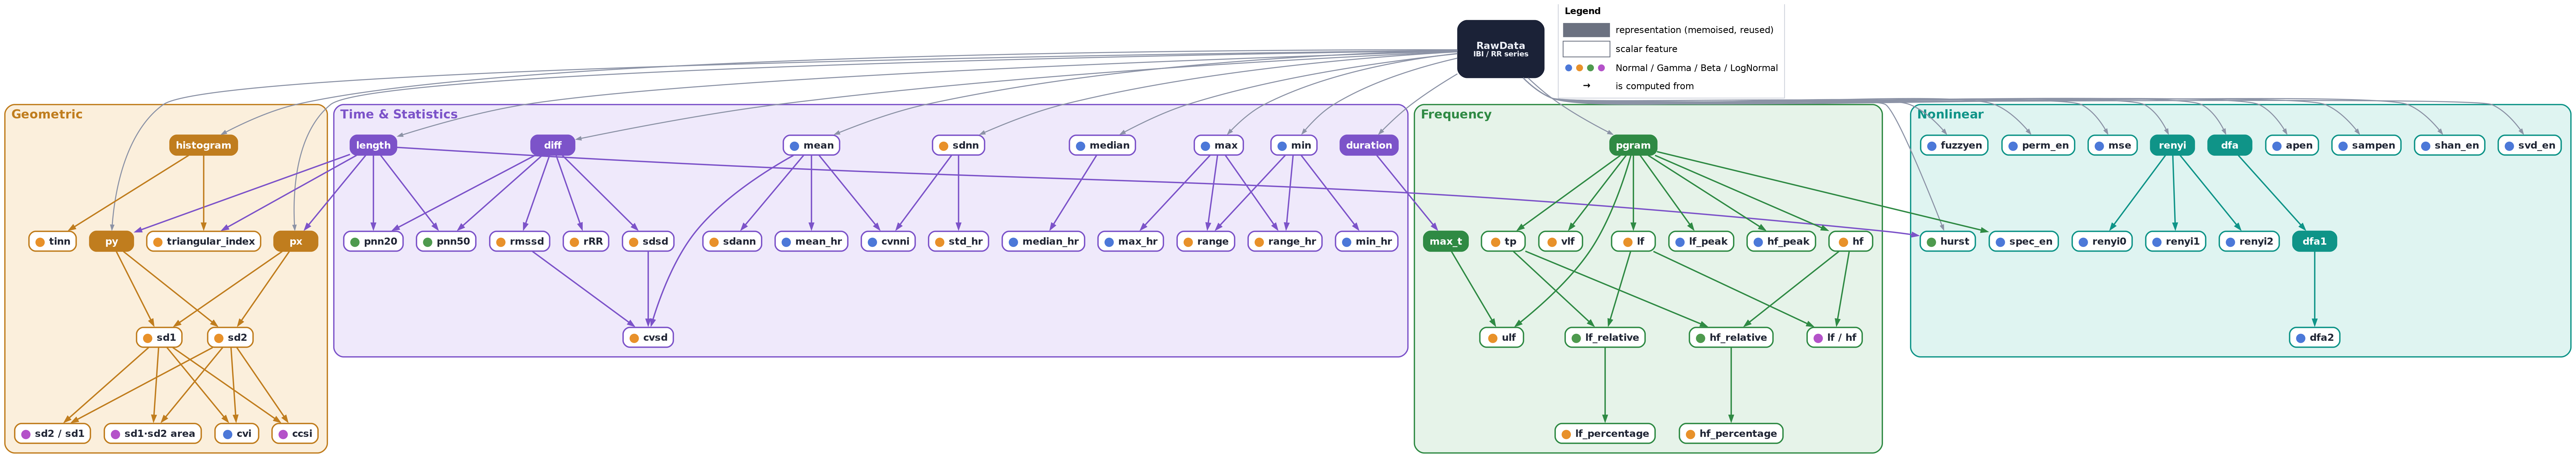
\includegraphics[width=0.92\linewidth]{figs/computational_graph.png}
  \par\vspace{1.5mm}
  {\raggedright\normalsize\color{inkdark}
   HRV features are \textbf{not independent measurements}. One IBI series feeds \textbf{11 memoised
   representations} which feed \textbf{53 scalar features}; every arrow is an ``is computed from''
   dependency read from the live \texttt{Features.jl} registry. RMSSD, SD1 and SDSD are the \emph{same}
   quantity up to a constant; LF/HF, LF\% and LF-rel are all functions of LF and HF: reporting them
   as independent evidence multiplies one fact, the \textbf{definitional} root of the empirical
   redundancy the clustermap shows below.\par}
\end{tcolorbox}

\vspace{2mm}

% ================= METHOD + PIPELINE =================
\begin{tcolorbox}[card, borderline west={5mm}{0mm}{jupurple}]
  \ctitle[jupurple]{Method}
  \begin{minipage}[t]{0.66\linewidth}\large
   \textbf{Read} IBIs $\rightarrow$ \textbf{preprocess} (bio-outliers, ectopic \& zero beats)
   $\rightarrow$ \textbf{53 HRV features} (time / frequency / geometric / nonlinear)
   $\rightarrow$ \textbf{window} (360 beats / 120 stride) $\rightarrow$ fit a \textbf{normative prior}
   per feature (Normal / Gamma / Beta / LogNormal) by MLE over \textbf{61{,}715 windows from 66 healthy
   subjects} $\rightarrow$ \textbf{score}: percentile $=F_{\text{prior}}(x)$,
   $z=\Phi^{-1}(\text{percentile})$.
  \end{minipage}\hfill
  \begin{minipage}[t]{0.32\linewidth}\normalsize\color{inkdark}
   {\color{jcpurple}\bfseries Scope.} Priors are MLE approximations (KS-rejected at n\,=\,56k); a $z$
   is a percentile re-expressed on a standard normal, window-level and descriptive.
  \end{minipage}
  \par\vspace{3mm}
  \centering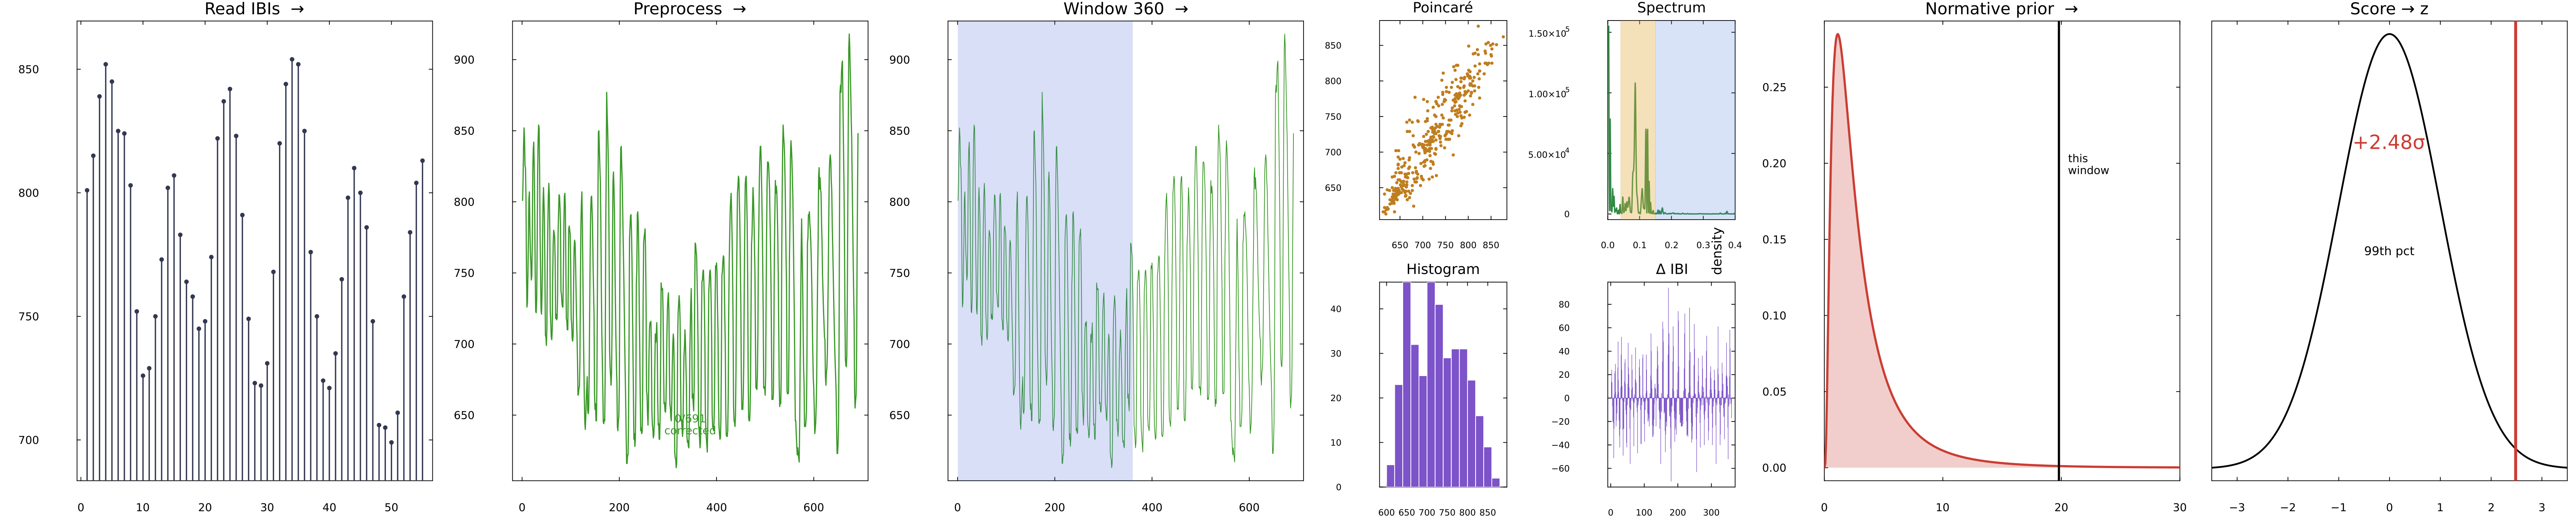
\includegraphics[width=0.995\linewidth]{figs/pipeline_chain.png}
  \par\vspace{1mm}
  {\small\color{inkdark} One real recording (Participant~P1) through every step. \textbf{Features}
  spans all domains (Poincar\'e, spectrum, histogram, successive differences $\to$ 53 numbers); here
  the window's LF/HF lands at the 99th percentile of the healthy prior ($z=+2.5$).}
\end{tcolorbox}

\vspace{2mm}
{\color{white}\bfseries\huge Results}\\[3mm]

% ── Feature analysis: clustermap + stability (swapped order) ──
\begin{tcbraster}[raster columns=2, raster column skip=8mm, raster equal height=rows]
  \begin{tcolorbox}[card, borderline west={5mm}{0mm}{jupurple}]
    \ctitle[jupurple]{HRV features are largely redundant}
    \centering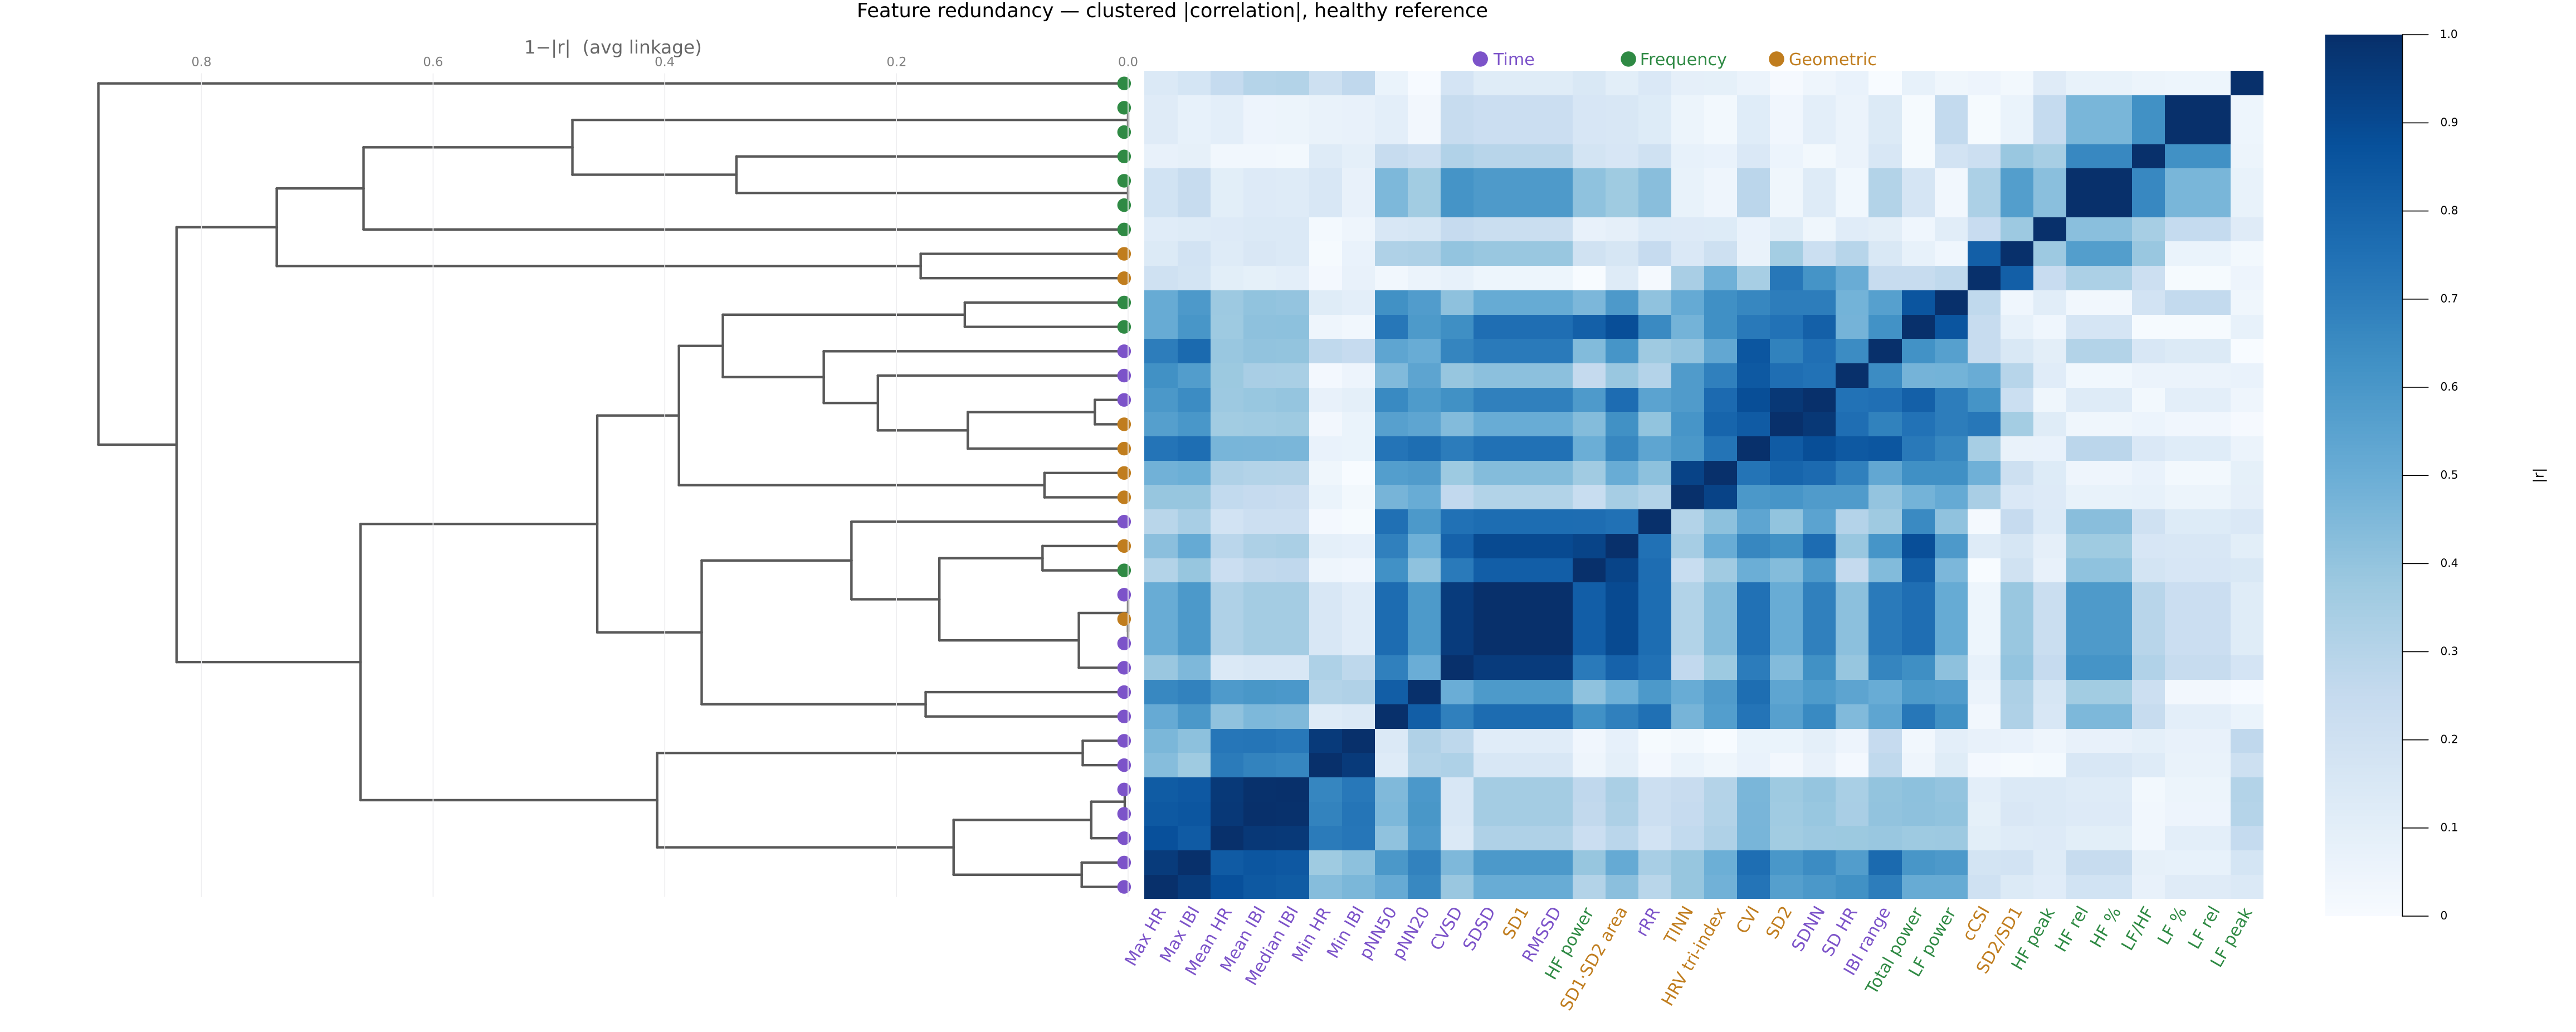
\includegraphics[height=123mm]{figs/feature_clustermap.png}
    \par\vspace{1mm}
    {\raggedright\normalsize\color{inkdark} Clustered $|$correlation$|$ on the healthy reference; the
    dendrogram groups near-duplicates. Dark blocks: SD1$\equiv$RMSSD$\equiv$SDSD ($r=1.00$),
    LF\%$\equiv$LF-rel, SDNN$\approx$SD2 \par}
  \end{tcolorbox}
  \begin{tcolorbox}[card, borderline west={5mm}{0mm}{jcgreen}]
    \ctitle[jcgreen]{Which features distinguish meditation}
    \centering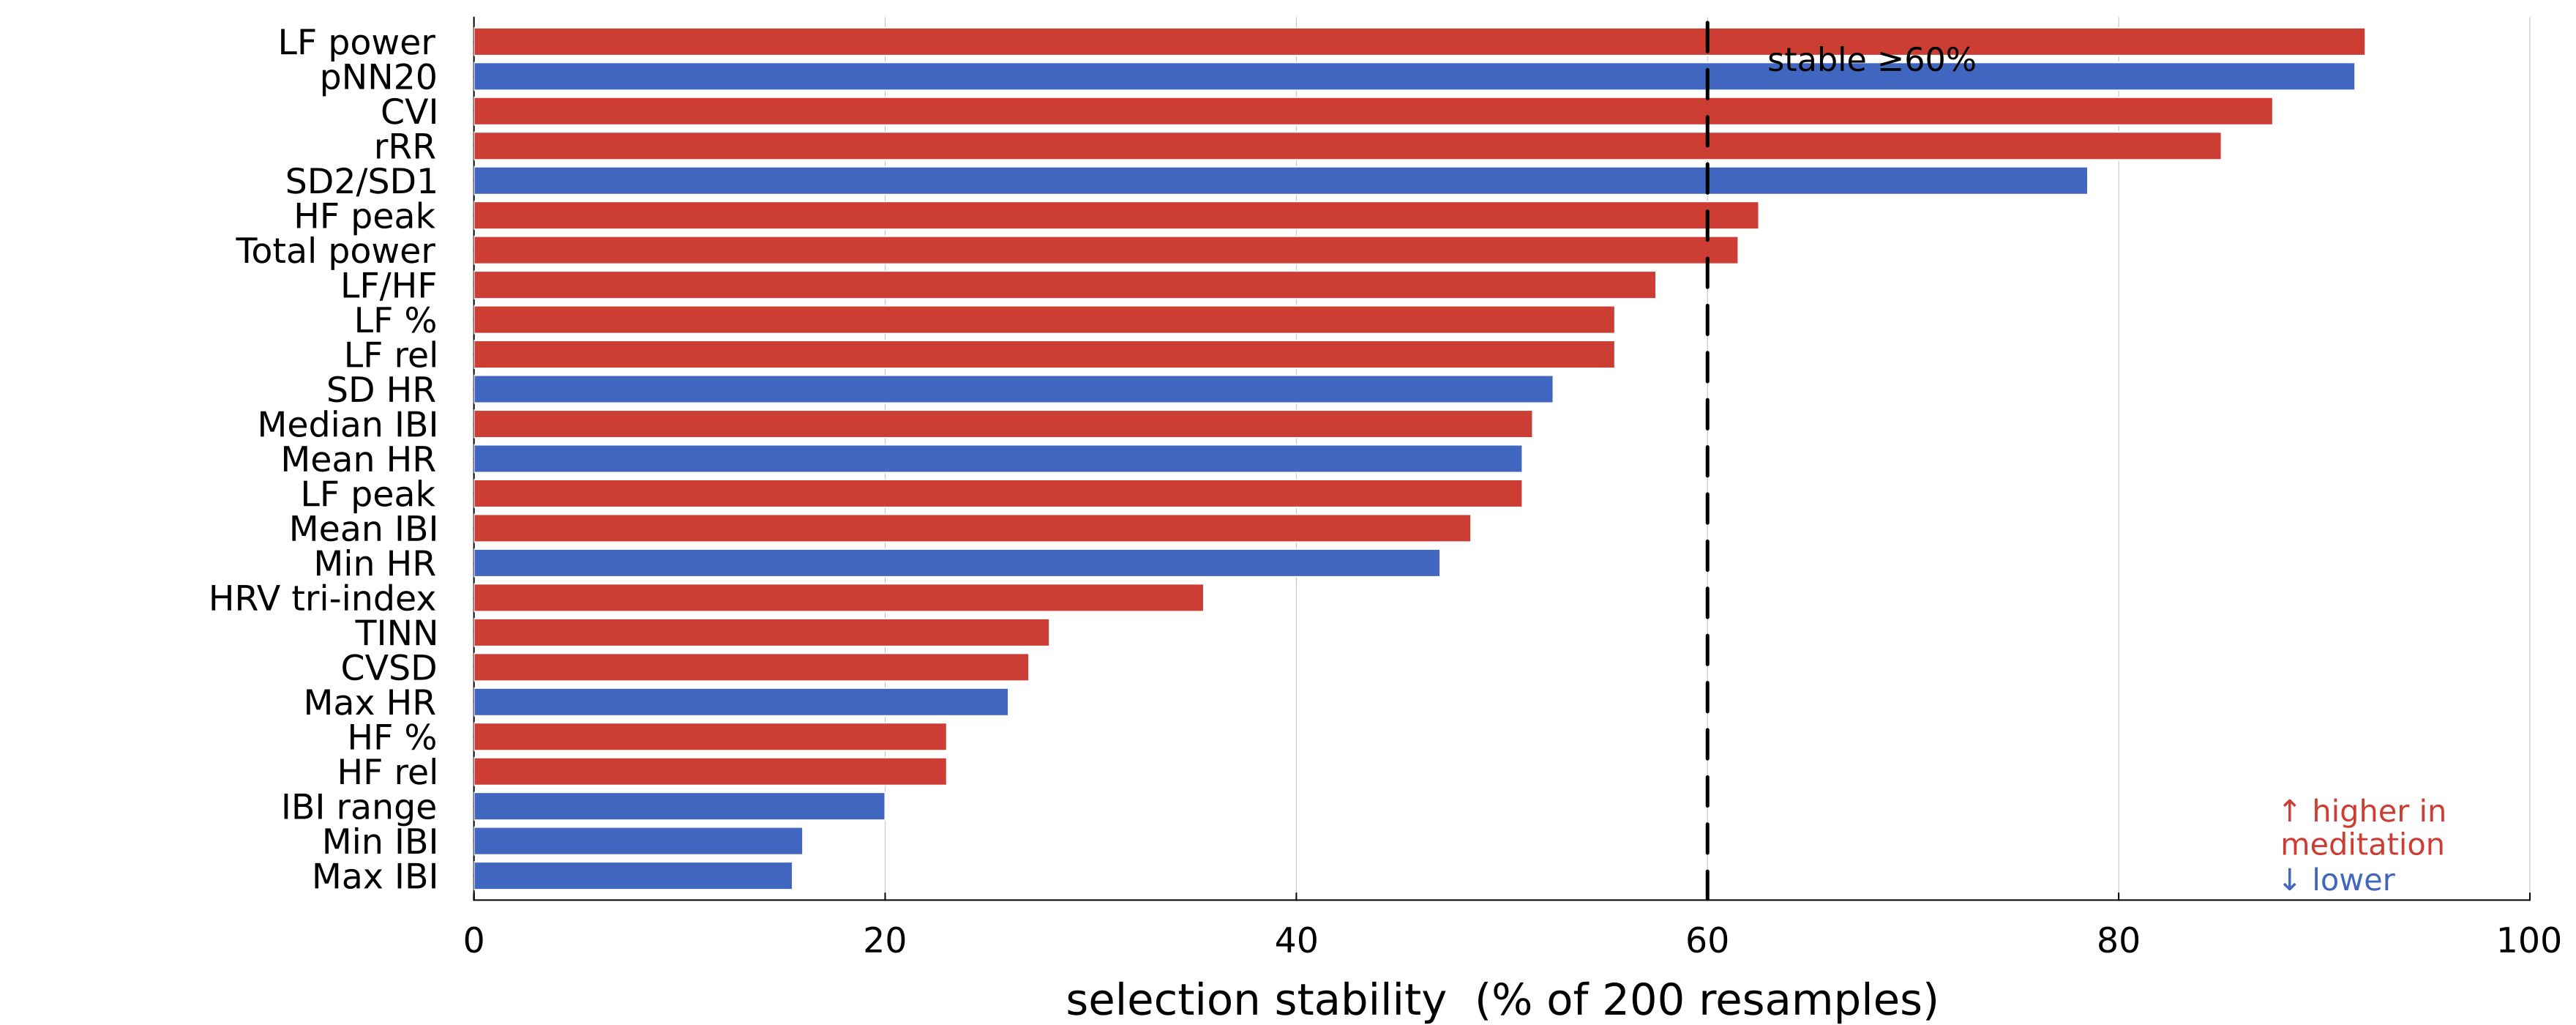
\includegraphics[height=123mm]{figs/stability_selection.png}
    \par\vspace{1mm}
    {\raggedright\normalsize\color{inkdark} L1-logistic \textbf{stability selection} (meditation vs
    healthy, 200 subject-grouped resamples): the $\sim$0.1\,Hz LF-band features are selected most
    often. Grouped 5-fold CV \textbf{AUC $=0.73\pm0.27$} (only 11 meditators). Features are
    chosen by the model.\par}
  \end{tcolorbox}
\end{tcbraster}

\vspace{1mm}

% ── Participant + population ──
\begin{tcbraster}[raster columns=2, raster column skip=8mm, raster equal height=rows]
  \begin{tcolorbox}[card, borderline west={5mm}{0mm}{jured}]
    \ctitle[jured]{Participant P1 scored against two references}
    \centering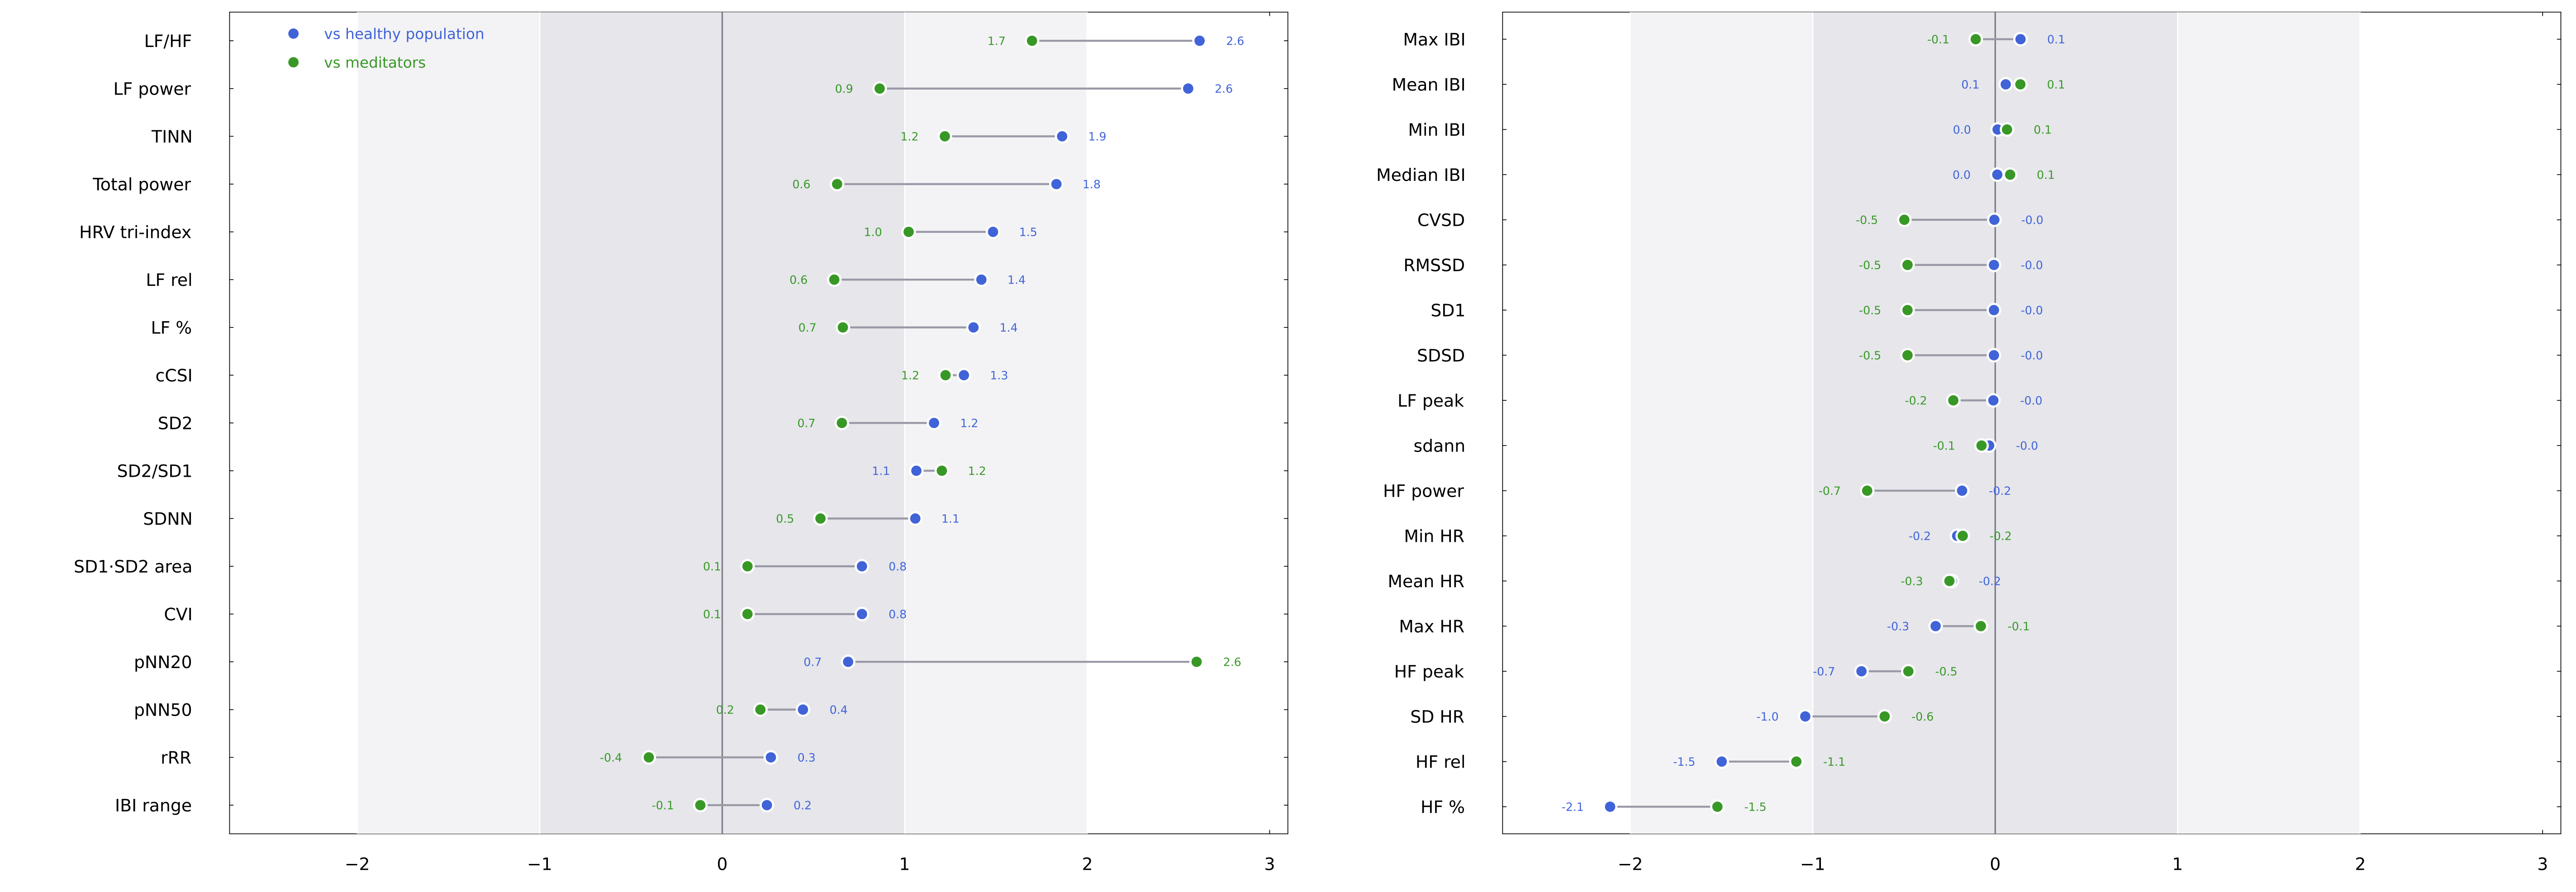
\includegraphics[width=\linewidth]{figs/zopt_2col.png}
    \par\vspace{1mm}
    {\raggedright\normalsize\color{inkdark} P1's deviation ($\sigma$-equivalent) from the
    \textcolor{jublue}{\textbf{healthy population}} and from the
    \textcolor{jcgreen}{\textbf{meditators}}. On the LF-band features P1 is extreme vs the general
    population (LF/HF $+2.6\sigma$) but close to a typical meditator ($+1.7\sigma$)\par}
  \end{tcolorbox}
  \begin{tcolorbox}[card, borderline west={5mm}{0mm}{jublue}]
    \ctitle[jublue]{Distributions: population, meditators, participant}
    \centering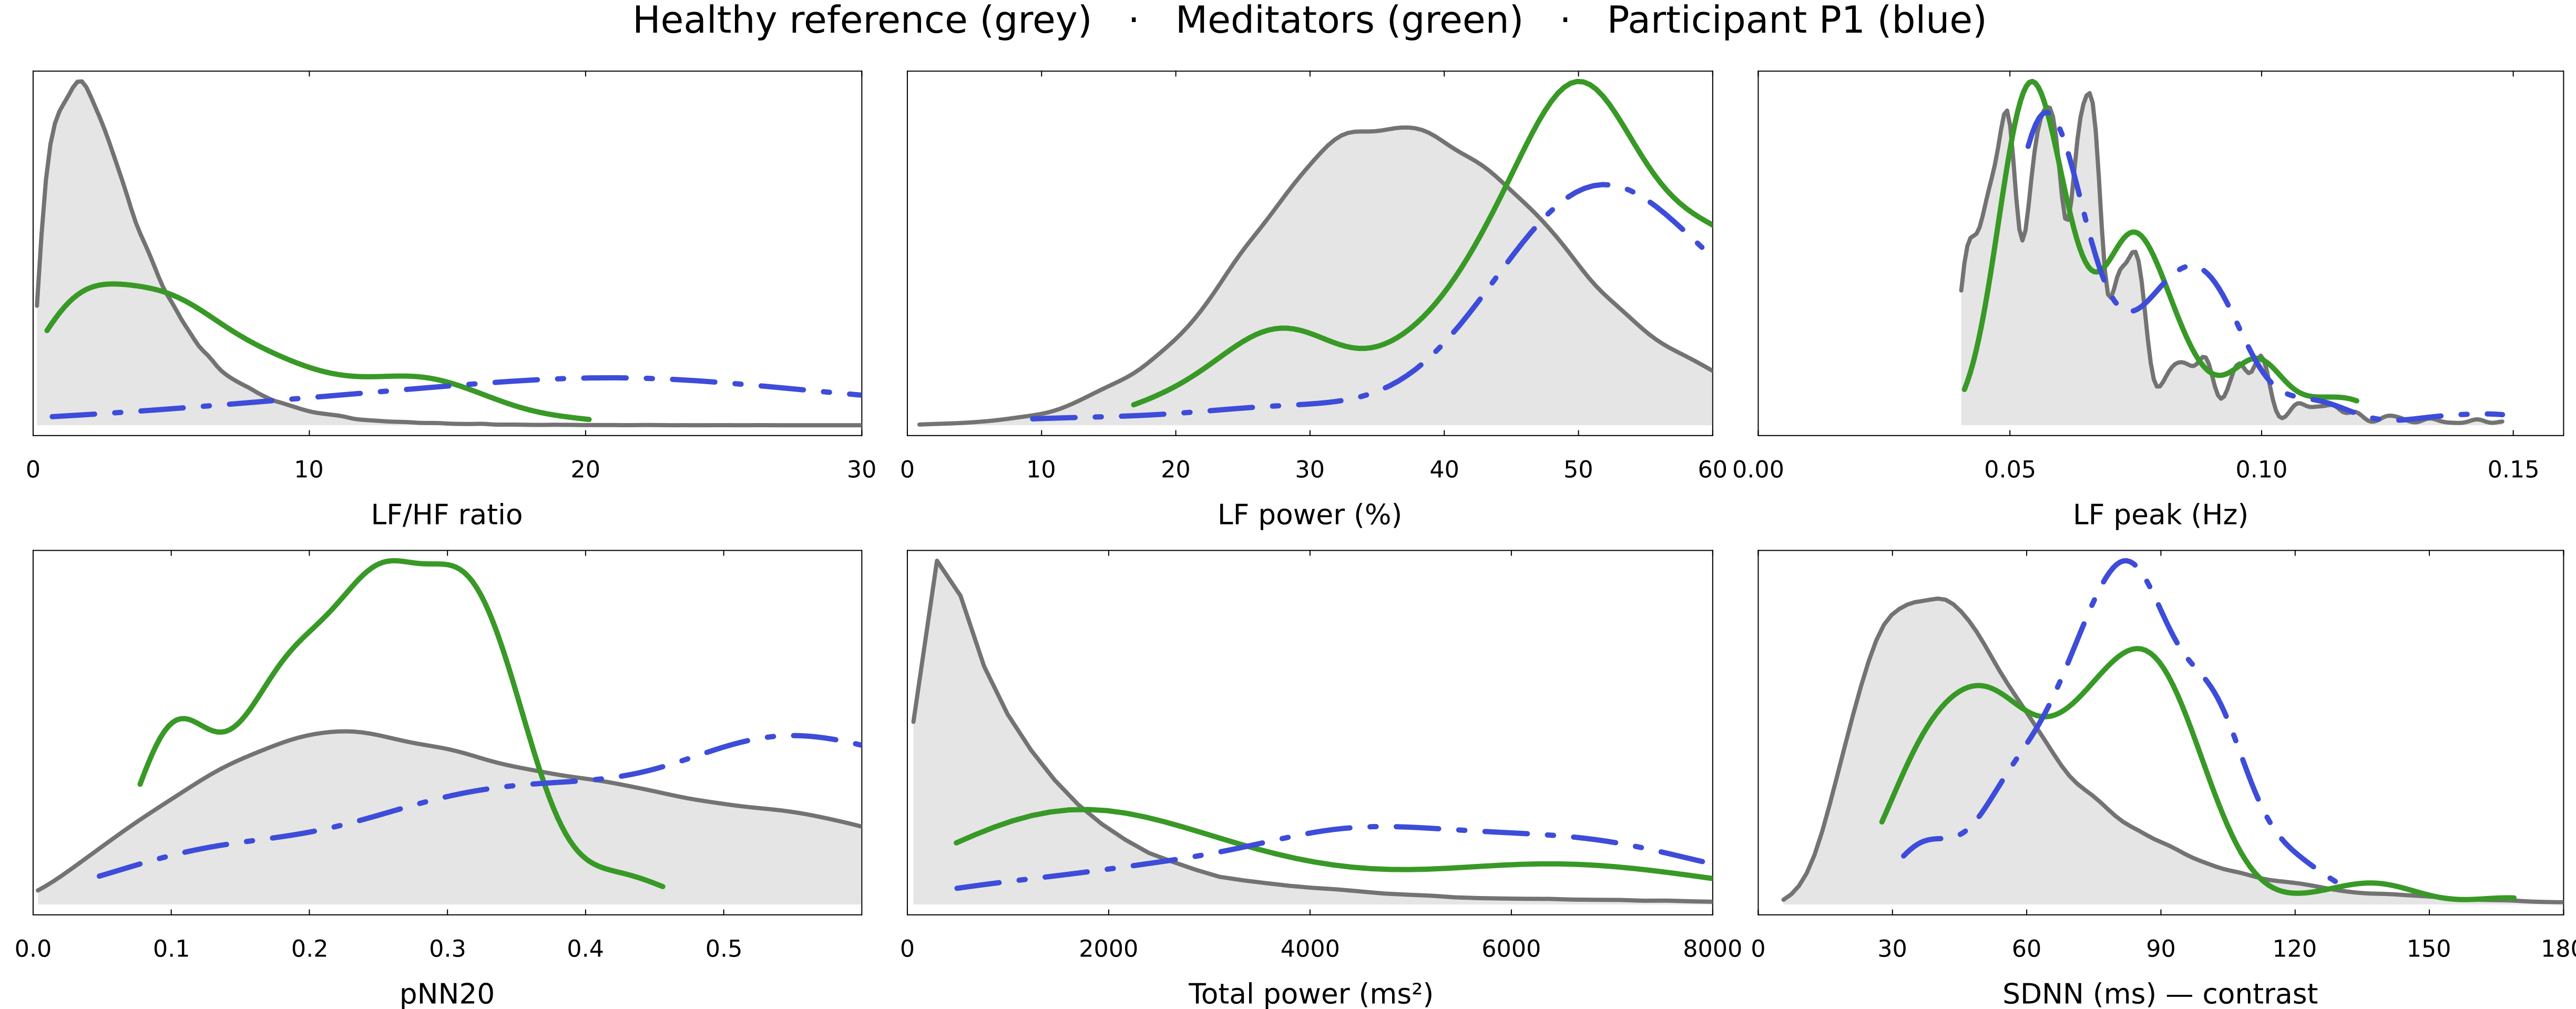
\includegraphics[height=123mm]{figs/three_way_comparison.png}
    \par\vspace{1mm}
    {\raggedright\normalsize\color{inkdark} \textcolor{gray}{\textbf{Grey}} = healthy reference (66
    subjects); \textcolor{jcgreen}{\textbf{green}} = meditators (11 practitioners);
    \textcolor{jublue}{\textbf{blue}} = P1. Both meditators and P1 shift the LF-band features right of
    healthy; short-term time-domain spread (SDNN) separates them much less.\par}
  \end{tcolorbox}
\end{tcbraster}

\vspace{2mm}

% ==================== TAKEAWAY + LIMITS =================
\begin{tcolorbox}[enhanced,colback=jcgreen,colframe=jcgreen,arc=6mm,
     fontupper=\color{white},drop fuzzy shadow=black!45,top=5mm,bottom=5mm,left=9mm,right=9mm]
  \begin{minipage}[t]{0.605\linewidth}
    {\bfseries\LARGE ``Is this new experimental data normal?''}\par\vspace{2.5mm}
    {\large HeartRateLab.jl answers it \textbf{only in context}. Participant~P1 (paced
    \textbf{resonant breathing}) reads as \textbf{atypical} against the general population
    (LF/HF $+2.6\sigma$) yet \textbf{meditator-like} against the meditation cohort
    (LF/HF $+1.7\sigma$). The \emph{same} recording has two verdicts, while the meditators
    themselves sit $<\!1\sigma$ from healthy. The contribution is the \textbf{framing}:
    placing one recording in a normative context, not statistical inference on P1.}
  \end{minipage}\hfill
  \begin{minipage}[t]{0.355\linewidth}
    {\color{white}\bfseries\Large Limitations}\par\vspace{2.5mm}
    {\normalsize\color{white!90} The ``normative'' references are convenience datasets
    (nsrdb/nsr2db), not sampled normal populations; per-feature priors are KS-rejected
    approximations; windows are correlated (descriptive, not inferential); the meditation
    cohort is n\,=\,11; \textbf{P1 is a single self-tracked participant}. Full detail and the
    feature table are in the notes handout.}
  \end{minipage}
\end{tcolorbox}


% ================= FOOTER (on lavender band) =================
\vfill
% Logos row: HeartRateLab (left) + institutional (right), SAME height, above the JuliaCon footer
\raisebox{-0.5\height}{
\includegraphics[height=22mm]{figs/hrl_logo_side_dark.png}}\hfill
\raisebox{-0.5\height}{
\includegraphics[height=22mm]{figs/inst_lasalle.png}}\hspace{9mm}%
\raisebox{-0.5\height}{
\includegraphics[height=24mm]{figs/inst_tu.png}}\hspace{9mm}%
\raisebox{-0.5\height}{
\includegraphics[height=25mm]{figs/inst_mu.pdf}}%
\par\vspace{2mm}
% ---- JuliaCon / venue / repo footer (restored) ----
\begin{minipage}[b]{0.34\linewidth}
   \raisebox{-1mm}{\juliadots{0.9}}\hspace{3mm}%
   {\color{inkdark}\bfseries\fontsize{46}{48}\selectfont julia}%
   {\color{jupurple}\bfseries\fontsize{46}{48}\selectfont con}\\[1mm]
   {\color{inkdark}\bfseries\Large Global\ \textcolor{jublue}{\textbullet}\ 2026}
\end{minipage}\hfill
\begin{minipage}[b]{0.36\linewidth}\centering
   {\color{inkdark}\bfseries\LARGE Johannes Gutenberg University}\\[1mm]
   {\color{jured}\bfseries\Large Mainz, Germany \; · \; August 10--15, 2026}
\end{minipage}\hfill
\begin{minipage}[b]{0.26\linewidth}\raggedleft
   {\color{inkdark}\large\faGithub~\textbf{abcsds/HeartRateLab.jl}}\\[1mm]
   {\color{jcpurple}\large Open data · Open source · Julia 1.11}
\end{minipage}

\end{document}
